\documentclass{llncs}
% packages should be added as needed 
\usepackage{graphicx}

\usepackage{algorithm} % for algorithms
%\usepackage{mathtools}

\usepackage{algpseudocode}
\algblockdefx[Process]{Process}{EndProcess}[2][Unknown]{{\bf Process} {\it #2}}{}
\algblockdefx[Event]{Event}{EndEvent}[2][Unknown]{{\bf upon event #2 do}}{}

\usepackage{booktabs} % For formal tables
\usepackage{cite} %for multiple refs

\usepackage{amssymb} %for nice emptyset

\usepackage[T1]{fontenc}
\usepackage{inconsolata}

\usepackage{color}

\definecolor{pblue}{rgb}{0.13,0.13,1}
\definecolor{pgreen}{rgb}{0,0.5,0}
\definecolor{pred}{rgb}{0.9,0,0}
\definecolor{pgrey}{rgb}{0.46,0.45,0.48}

\usepackage{listings}
\lstset{language=Java,
  showspaces=false,
  showtabs=false,
  breaklines=true,
  showstringspaces=false,
  breakatwhitespace=true,
  commentstyle=\color{pgreen},
  keywordstyle=\color{pblue},
  stringstyle=\color{pred},
  basicstyle=\ttfamily,
  moredelim=[il][\textcolor{pgrey}]{$$},
  moredelim=[is][\textcolor{pgrey}]{\%\%}{\%\%}
}

%\usepackage{amsthm} % For claims
%\theoremstyle{remark}

%\settopmatter{printacmref=false, printccs=false, printfolios=false}
\pagestyle{plain} % removes running headers

\newcommand{\PicScale}{0.5}
\newcommand {\FlameStream} {FlameStream}
\begin{document}

\title {Deterministic model for distributed speculative stream processing}
\author{Igor E. Kuralenok\inst{1}
       \and Artem Trofimov\inst{1,2}\orcidID{0000-0002-8916-9659}
       \and \\Nikita Marshalkin\inst{1,2}\orcidID{0000-0002-7273-1692}
      \and Boris~Novikov\inst{1,2}\orcidID{0000-0003-4657-0757}}
\institute{JetBrains Research, St. Petersburg, Russia \and
     Saint Petersburg State University, St. Petersburg, Russia  \\
\email{\string{ikuralenok, trofimov9artem, marnikitta\string}@gmail.com, borisnov@acm.org}
}

\maketitle

\begin{abstract}
Users of modern distributed stream processing systems have to choose between non-deterministic computations and high latency due to a need in excessive buffering. 
%In addition, a sophisticated state management must be implemented at the business logic level to provide fault tolerance. 
We introduce a speculative model based on MapReduce-complete set of operations that allows us to achieve determinism and low-latency.
Experiments show that our prototype can outperform existing solutions due to low overhead of optimistic synchronization.

%In recent years, there has been a growth in research and industrial solutions in the field of distributed stream processing. 
%However, even state-of-the-art stream processing systems are inconvenient to work with in some ways. 
%Firstly, existing solutions suppose that the state of operations should be managed directly by a user, and that can be confusingly for inexperienced users of analytical processing systems. 
%Secondly, these systems do not provide for deterministic processing by default. 
%Furthermore, the most common approach for this feature is buffering. 
%Its main problem is the extra cost for blocking before each order-sensitive operation. 
%The goal of this paper is to propose a model, which addresses both recognized issues. 
%On the one hand, our model stateless from the business logic perspective. 
%Such behavior is obtained by the technique that allows a state to be a part of a stream. 
%On the other hand, it is deterministic by design. 
%We introduce an optimistic method that avoids buffering before each operation to achieve determinism with low overhead. 
%The experiments show that prototype of our system requires a low extra cost for supporting proposed features and is able to outperform alternative industrial solutions in certain conditions.

\keywords{Data streams \and Distributed processing \and Drifting state.}
\end {abstract}

\section {Introduction}
%%% fs-run-time-intro  - Introduction

\label {fs-intro-seciton}

A need to process huge amounts of data (e.g. Internet scale) was addressed by scalable distributed data processing systems such as  mapreduce. These systems are able to run data processing in a massively parallel mode on a clusters consisting of thousands of commodity computers. 

However, the initial models and frchitectures of this kind suffered from several drawbacks deeply analyzed in~\cite{Doulkeridis:2014:SLA:2628707.2628782,}. Many of these drawbacks were addressed in the next generation of scalable distributed data processing architectures, e.g. 
Asterix~\cite{Alsubaiee:2012:ASW:2331801.2331803}, 
Spark~\cite{Zaharia:2016:ASU:3013530.2934664,Franklin:2015:MSB:2684822.2685326}, 
and Flink~\cite{Carbone:2017:SMA:3137765.3137777}. 

The goal of the FlameStream (how should it be written? with a space or like here?) is to further improve performance and provide for better consistency of the output.  Specifically, the objectives are:

\begin {itemize}
\item ready on key: the output is delivered as soon as it is computed for every single key, rather than at the completion of  the whole workflow.
\item exactly once execution: each input item is processed exactly once even in case of partial system failures. 
\end {itemize}

A brief outline of the overall architecture and planned features: types, declarative workflow specification, ? ? ?

This paper introduces a run-time module of the  FlameStream. 
Add more details here.

The contributions of this paper are the following:

\begin {itemize}
\item definition of the computational model
\item implementation and proof of the concept.
\end {itemize}

The rest of the paper is structured as follows 
Describe sections here: model~\ref {fs-model-section}
implementation~\ref{fs-implementation-section}
experiments ~\ref{fs-experiments-section}
related work~\ref{fs-related-section}.


\endinput


\section {Model}
\label {fs-model}

\subsection {Motivation}
%%%% fs-run-time-motivation  FlameStream motivation

\label{motivation-section}

Implementation of deterministic processing is tightly connected to system state management: if user-defined operations are pure functions and the total order is preserved, the processing becomes deterministic. Most of existing stream processing systems have been already supposing that user-defined operations are pure. Instead of providing a handler for external storage they give user operation the state object, provide the user an interface to change the state and finally store the resulting state object after the operation completes~\cite{carbone2015apache, apache:storm, Noghabi:2017:SSS:3137765.3137770}.

Let $B$ denote a business logic operation, $x \in \mathbb{E}, Y \subset \mathbb{E}$ be input and output items, $h$, the state handler and $s_t$, the state object at time $t$. The change in contract is illustrated in (\ref{flink-contract}). In modern setting $B$ becomes stateless and state management is done on the system side. This change allows the system to implement fault tolerance mechanisms, but it also opens the opportunity to implement deterministic processing.

\begin{equation}
\label{flink-contract}
Y = B(x, h) \Rightarrow (Y, s_t) = B(x, s_{t-1}) 
\end{equation}

The only difference between a state object $s_t$ and the other items in the stream is that state objects are produced, updated and consumed by the same operation. If a system allows cyclic execution graphs~\cite{Murray:2013:NTD:2517349.2522738} this difference becomes obsolete, as we can transfer state object from operations output to its input. We treat state object as a part of the stream and we call it {\it drifting state}. Drifting state allows moving fault tolerance logic from user-defined operations to common stream consistency mechanisms.

The second property of the system needed for deterministic processing is total order preservation. This one is quite challenging due to asynchronous nature of the network. On the other hand, we need to care about the order only in the operations that are order-sensitive. All stateless operations are tolerant to the out-of-order items. The more stateless operations we have, the easier the task becomes. Another important note is that calculations are partitioned, and order between items from different partitions does not influence the result. Partition could be calculated at single compute unit, which allows us to implement ordering within single unit instead of system-wide.

Taking into account above considerations we think that 
modern stream processing problem setup allows us to build a system that can provide deterministic processing with low-performance overhead. The desired system properties are:
\begin{itemize}
    \item Computational model should be deterministic by design, i.e., it should produce deterministic results for any pipelines and business logic.
    \item The performance overhead should be low in comparison with the existing systems.
\end{itemize}
We will use the following principles for our system:
\begin{itemize}
    \item Support cyclic execution graph
    \item Localize state management in terms of system operation type
    \item A data partition must be processed on a single node
    \item MapReduce completeness
\end{itemize}


\subsection {Computational model}
%%%% fs-run-time-data-flow  FlameStream data flow

\label {fs-model}

The key concept of \FlameStream\ model is a datastream. It is a sequence of discrete events described by data items, internally represented as 
$(Payload, Meta).$
The $payload$ is processed by a  user-defined code, while $Meta$ is handled with \FlameStream\ engine. In particular
the primary purpose of the meta-information is to impose the total order on data items. 
The  $Meta$ is assigned at the entry (called {\em  front}) and is discared at the {\em barrier} just before the exit. 

% \subsection{Computational flow}
The stream processing is specified by a logical execution graph. 
Each node of the graph represents a single operation on data items, and edges describe the routing of data items between operations.  
Our model allows cycles in the graph while such graphs are commonly assumed to be acyclic (DAGs) 
~\cite{Zaharia:2016:ASU:3013530.2934664, Carbone:2017:SMA:3137765.3137777}. 
The cycles are required for specification of certain computations (e.g MapReduce-based) with our spartan set of operation types (outlined below).
%Moreover, as we show further, there are cases when cycles are required, e.g., for MapReduce-based algorithms. 
Figure~\ref{logical-graph-figure} shows the example of logical execution graph.

% \subsection{Physical deployment and partitioning}
A distributed hardware environment is modelled as a set of {\em worker} processes. 
Each the workers executes logical execution graph and has an assigned range of hash values used for physical routing of data items to workers. 
%An integer interval (hash range) is assigned to every worker. Intervals are not intersected and cover the range of 32-bit signed integer.
%
Each operation input has a user-provided hash function called {\it balancing function}. This function is applied to the payload of data items and determines partitioning before each operation. After that, the data items are sent to the worker, which is responsible for the associated hash range. Therefore, load balancing explicitly depends on the user-defined balancing functions. 
%This allows the developer to determine optimal balancing which requires the knowledge of the payload distribution. The system optimizes the hash ranges assignment according to the processing statistics. 

\begin{figure}[ht]
  \centering
  \begin{minipage}[b]{.5\textwidth}
    \centering
    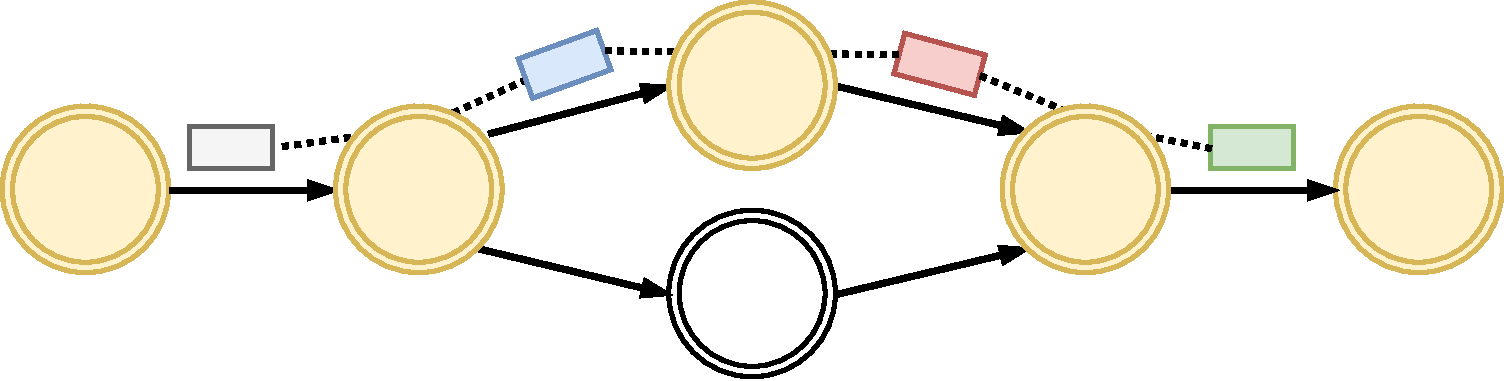
\includegraphics[width=0.9\linewidth]{pics/logical-graph}
    \caption{A logical execution  graph}
    \label{logical-graph-figure}
  \end{minipage}%
  \begin{minipage}[b]{.5\textwidth}
    \centering
    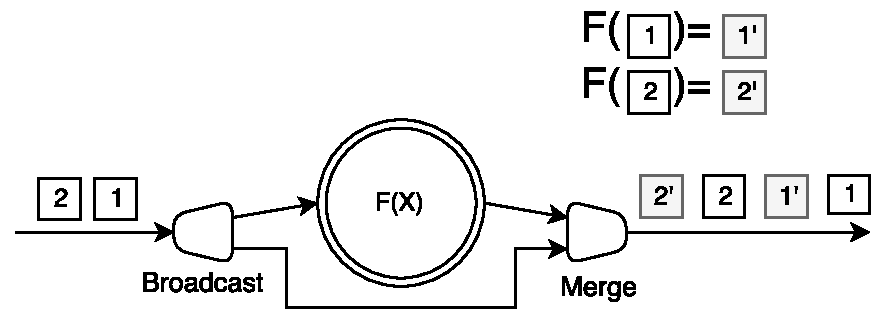
\includegraphics[width=\linewidth]{pics/ordering}
    \caption{The ordering model}
    \label{ordering}
  \end{minipage}
\end{figure}

% мм\subsection{Ordering model}

Data items are totally ordered according to lables assigned to events at the entry as a part of meta-information. All operations preserve this order. Any additional items produced by an operation are placed between the item being processed and the next item. The ordering labels are dropped when items are delivered from the barrier. 

% We assume that there is a total order on data items. 
% Ordering is preserved when an item is going through the operations. 
% More precisely, the order of output items is the same as the order of corresponding input items. 
% If more than one item is generated, they are inserted in output stream sequentially. 
% Moreover, the output follows corresponding input but precedes the next item. 
% Without diving into details, it should be noted that the order of items is maintained across different fronts.

The ordering is illustrated  in Figure~\ref{ordering}. Data item with payload $1'$ is the derivative of the item with payload $1$, according to operation $F$. The same is for items with payloads $2'$ and $2$. After merge operation, the order between $1$ and $2$ is preserved. Furthermore, $1'$ follows $1$, and $2'$ follows $2$.  

%  We assume that input items of the operations are strictly ordered.

%  \subsection{Operations}

The list of available operations includes:
\begin {description}
\item [Map] applies a user-defined function to the payload of an input item and returns a (possibly empty) sequence of data items with transformed payloads. 

\item [Broadcast] replicates an input item to the specified number of operations.

\item [ Merge] operation is initialized with the specified number of input nodes. It sends all incoming data to the output.

\item [ Grouping]  constructs a single item containing a set of consequtive items assigned to the same worker. The maximem nuber of items that can be grouped is specified as a parameter and is called window size. 
\end {description}

Grouping is the only operation that has a state.

%has a {\it window size} parameter. Grouping stores input items into distinct buckets by the value of the input balancing function applied to the payload. When the next item arrives at the grouping, it is appended to the corresponding bucket. Each time the grouping outputs window-sized {\it tuple item}, which consists of the most recent (in terms of the meta-information) items of this bucket. If the size of the bucket is less than the window, all items of the bucket are taken. 

The following example illustrates the semantics of the operation. The grouping accepts items with payload represented as natural numbers: 1,2,3, etc. The load balancing function returns 1 if the number is even and 0 otherwise. If the window is set to 3, the output is: \[(1), (2), (1|3), (2|4), (1|3|5), (2|4|6), (3|5|7), (4|6|8)...\]

The grouping operation has  two important properties: the output tuple is identified by its last element, the results among items with different values of a hash function are independent.

% \subsection{User-defined parameters}

% A user can set up the following parameters:

% \begin{enumerate}
%  \item{Computational flow}
%  \item{Balancing functions of the inputs}
%  \item{Map functions}
%  \item{Grouping windows}
%\end{enumerate}

%These parameters can produce more than one graph, which can yield equivalent results. Choosing among them is a performance optimization problem that relies on the system.
%It is important to mention that there are no parameters for state-management. 
%Therefore, business-logic is stateless. Nevertheless, the operations set is enough to implement any MapReduce transformation as shown in the next section.


 \subsection{Drifting state}
 %% It is just an empty TeX file.
%% Write your code here.

\label{fs-drifting}

Add bla-bla.

\subsection{MapReduce transformation}

TODO: rewrite. In this section, we demonstrate possible implementation of MapReduce-like transformation on a stream in order to show the soundness of our model. Map stage can be formulated in terms of our map operation. However, it is not obvious how to implement reduce stage, because it requires an explicit state handling. The algorithm~\ref{reduce} shows a generic reduce stage. The {\it accumulator} is an explicit state that should be maintained between subsequent iterations.

\begin{algorithm}
\caption{Generic reduce stage}
\label{reduce}
\begin{algorithmic}
  \Function{reduce}{$key$, $values$}
    \State $accumulator$ \Comment{reduce's state}
    \ForAll{$v \in values$} 
      \State \Call{combine}{$v$, $accumulator$}
    \EndFor
    \State \Return \Call{map}{$accumulator$}
  \EndFunction
\end{algorithmic}
\end{algorithm}

One possible way to implement reduce stage in our model is to make business logic state a part of the stream and work with it like with an ordinary data item. Figure~\ref{mapreduce-graph-figure} shows a generic graph for MapReduce transformation. Map and reduce parts are highlighted with a dashed line.

\begin{figure}[htb]
  \centering
  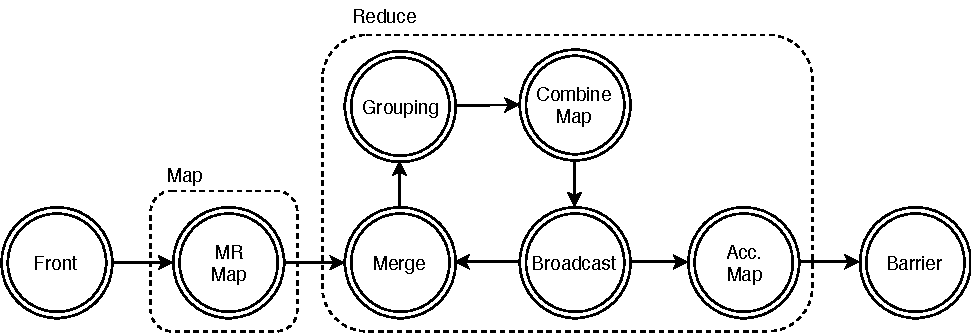
\includegraphics[scale=0.5]{pics/mapreduce}
  \caption{Logical graph for MapReduce transformations}
  \label {mapreduce-graph-figure}
\end{figure}

There are four types of data items in this stream: {\it input}, {\it mapped}, {\it accumulator}, {\it and reduced} items. Mapped, accumulator, and reduced items have the key-value structure of a payload. The operations of the stream have the following purposes:

\begin{itemize}
  \item The first map operation accepts input items and outputs mapped items according to map stage of MapReduce model
  \item The window of grouping is set to 2. It is used to group current accumulator with next data item in order to combine them together further. The hash function is designed to return distinct values for payloads with distinct keys
  \item The second map implements the actual combining. It accepts inputs that have a form of: \textit{(mapped item)} or \textit{(accumulator item, mapped item)}. The first kind is transformed into some initial value. The second one is combined into the new accumulator item as specified by reduce stage of MapReduce. The tuples with structure \textit{(mapped item, accumulator item)} are filtered out
  \item The third map is the accumulator map. It accepts accumulator items and applies the final map transformation to them
\end{itemize}

The key idea is that ordering assumptions about data items guarantees that each accumulator item always arrives at the grouping right after previous mapped item and before a new one. Hence, each mapped item that has not been combined yet would be grouped with the right accumulator item. Additionally, when combine map accepts tuple {\it (mapped item, accumulator item)}, then it means that mapped item was generated before accumulator item, and therefore, it had been already combined. The cycle gives the ability for new accumulator items to get back in the grouping operation. The accumulator map transforms the accumulator item into the final reduced item right before sink. Thereby, the stream reacts to each input item by generating new reduced item, which contains the actual value of the reduce stage.

\subsection{Example: word count}

We illustrate the MapReduce algorithm with an example of word counting. Map stage of this algorithm transforms each input word into key-value pair where the word is a key, and the value is 1. Reduce stage sums all values into the final result for the specific key. In this case the accumulator map is omitted, because the accumulator is the actual result of the reduce stage.

The example of input/output items, which are generated/ transformed by the part of the logical graph, is shown in Figure~\ref {word-count-figure}. According to our graph for MapReduce transformations, the item {\it m[dog, 1]} represents mapped item with key "dog" and value 1. The item {\it a[dog, 1]} describes accumulator item with key "dog" and value 1. Figure shows how the model reacts on two consequent input items containing word "dog". The meta-information of items is omitted for simplification. More precisely, there are 4 stages separated by dotted lines:

\begin{enumerate}
    \item New mapped item with key "dog" arrives at grouping with an empty state. Grouping outputs tuple with this single item. Combine map transforms it into the first accumulator item for key "dog" and value 1.
    \item The accumulator item arrives at grouping after it went through the cycle. It is grouped in the tuple with the mapped item that has been already in the state with key "dog". However, combine map drops this tuple, because of the order of items.
    \item New mapped item with key "dog" arrives at grouping. It is inserted right after the accumulator in the bucket for key "dog". The grouping operation outputs tuple containing the accumulator item and new mapped item. Map operation combines reduced and mapped items into new reduced items with key "dog" and value 2.
    \item New accumulator item arrives at grouping through the cycle, but new generated tuple is not accepted by combine map, as well as in step 2.
\end{enumerate}

\begin{figure}[htb]
  \centering
  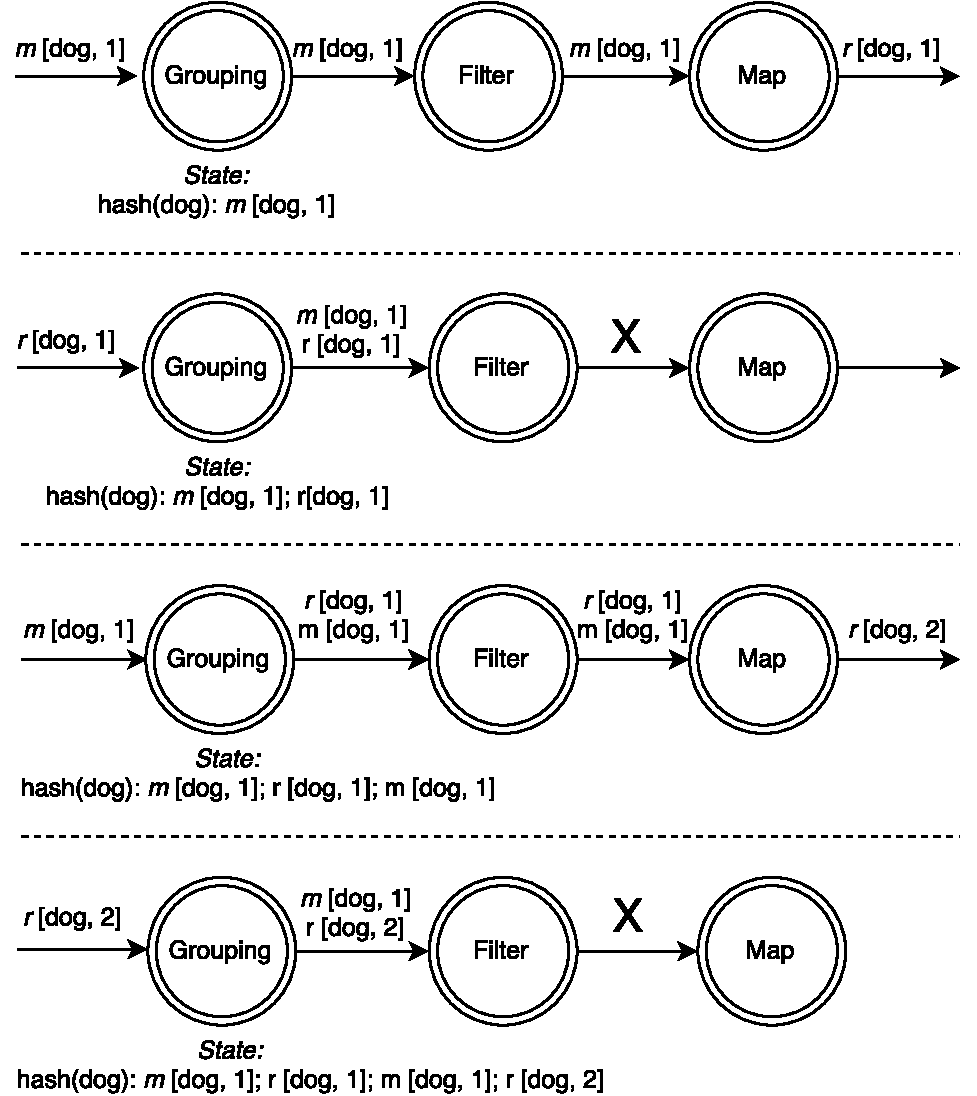
\includegraphics[scale=0.5]{pics/wordcount}
  \caption{Part of the stream evalutaion for word counting}
  \label {word-count-figure}
\end{figure}


\subsection {Deterministic computations}
%%%% fs-run-mapreduce Optimistic collision management
\label {fs-collision}

Deterministc execution is a desired property of any kind of system. If there are multiple possible outcomes, the developer needs to reason about which results are valid, which are equivalent and which are considered to be invalid.

To reduce outputs to only one possible result we impose two restrictions on our model: 

\begin{itemize}
  \item We require {\it map} function to be pure: return value is only determined by its input values, without observable side effects
  \item We impose a strict ordering requirements on the {\it grouping}'s input
\end{itemize}

While the first requiremet can be easily satisfied by moderating the provided business-logic, the second one is foreign to the distributed systems. Because of asynchrony and the possible existence of multiple paths between two nodes it is hard to deliver the right order. 

In this section we review common approaches for order enforcing, then we introduce our approach.

\subsection{Existing solutions}

There are two most common methods that are used to implement order-sensitive operators: in-order processing (IOP) \cite{Arasu:2006:CCQ:1146461.1146463, Cranor:2003:GSD:872757.872838, hammad2004optimizing} and out-of-order processing (OOP) \cite{Li:2008:OPN:1453856.1453890}.

According to IOP approach, each operation must enforce the total order on output elements that can be violated due to asynchronous nature of execution. Buffering is usually used to fulfill this requirement. For example, the implementation of the merge operator, in presence of a skew between input streams, must buffer the earlier one to enforce order on the output.

OOP is an approach that does not require order maintenance if it is not needed. In the case of ordering requirements, OOP buffers input items until a special condition is satisfied. This condition is supported by progress indicators such as punctuations \cite{Tucker:2003:EPS:776752.776780}, low watermarks \cite{Akidau:2013:MFS:2536222.2536229}, or heartbeats \cite{Srivastava:2004:FTM:1055558.1055596}. They go through the stream as ordinal items, but do not trigger business-logic of the operations. Each progress indicator carries meta-information and promises that there are no any elements with lesser meta-information. Therefore, indicators must be monotonic, but data items between two consecutive indicators can be arbitrarily reordered. Data sources periodically yield them.

While these methods are commonly adapted in practice we find them to have unpredictible latencies and to have bursty loads. In our system we employ an optimistic approach for handling out-of-order items.

\subsection{Optimistic approach}

In order to implement ordering model, we accept the fact that grouping can produce incorrect tuples. However, we guarantee that all correct tuples are eventually produced. The correctness of tuple means that this tuple would be generated if the order assumption was satisfied. 

To eventually produce all correct tuples, we use an approach called {\it replay}. If an item arrives the grouping operation, according to the meta-information order, nothing is replayed and only the most recent window is produced. However, if an item is out-of-order, it is inserted in the bucket at the correct location, and all tuples, which contain this element, are reproduced. Thereby, replay guarantees that eventually all correct tuples are generated. At the same time, for tuples, that has been produced but became invalid, {\it tombstones} are sent.

Tombstones are ordinal data items but with a special flag in its meta-information. This flag means that tuples with such meta-information are invalid, and they should not leave the system. Tombstones have the same payloads as invalid items in order to go along the same path in the computational pipeline.

The example of replay is shown in Figure~\ref{grouping-replaying}, The green item is out-of-order. The output consists of the new valid items {\it (1, 2) and (2, 3)}, and the tombstone {\it (1, 3)} for the previously generated item.

\begin{figure}[htbp]
  \centering
  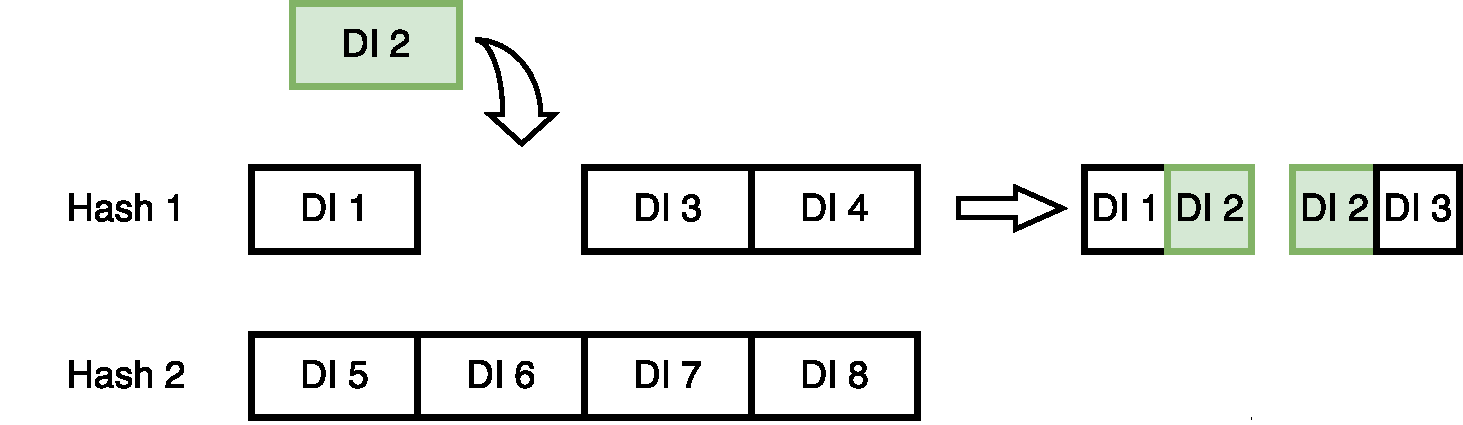
\includegraphics[width=0.48\textwidth]{pics/grouping-replaying}
  \caption{The replay in groupig with window = 2. The new items are generated on insertion}
  \label {grouping-replaying}
\end{figure}

In the case of the right order of input items, there are no redundant items produced.

The barrier filters out invalid elements, when corresponding tombstones arrive. It is partially flushed for some meta-information interval when there is a guarantee that there are no any out-of-order items and tombstones further up the stream for this range. The exact technique for providing such guarantee is defined in Section~\ref{fs-impl}.

\subsection{Advantages and limitations}

The proposed architecture's performance depends on how often reorderings are observed during the runtime. In the case when the order naturally preserved there is almost no overhead: when the watermark arrives, all computations are already done. The probability of reordering could be managed on a business-logic level and optimized by the developer. In experiments section it is shown that the computational nodes count is one of such parameters. Regarding the weaknesses, this method can generate additional items, which lead to extra network traffic and computations. Experiments, which are shown in the section~\ref{fs-experiments-section} demonstrate that the number of extra items is low.



\section {Implementation}
%%% fs-run-time-impl Implementation
\label{fs-impl}

\FlameStream\ is implemented in Java, using Akka framework for messaging. There are several main components within the implementation:
\begin{description}
  \item[Data producers and data consumers] are deployed separately and play the role of data source and data sink correspondingly.

  \item[Graph] is a component that is deployed on each node and executes a computational pipeline defined by a logical graph. Operations within the same node communicate with each other via direct function calls for performance optimization.

  \item[Barrier] filters out invalid data items. Besides, it delivers output items to data consumers.

  \item[Acker] tracks data items within the stream. Its functionality is detailed further.

  \item[Apache ZooKeeper] is used for cluster management. The usage of ZooKeeper mitigates the need for the dedicated master node.

  \item[Persistent storage] is needed for recovery in case of failures
\end{description}

The overall scheme of the system components is shown in Figure~\ref{system-architecture}.

\begin{figure}[ht]
  \centering
  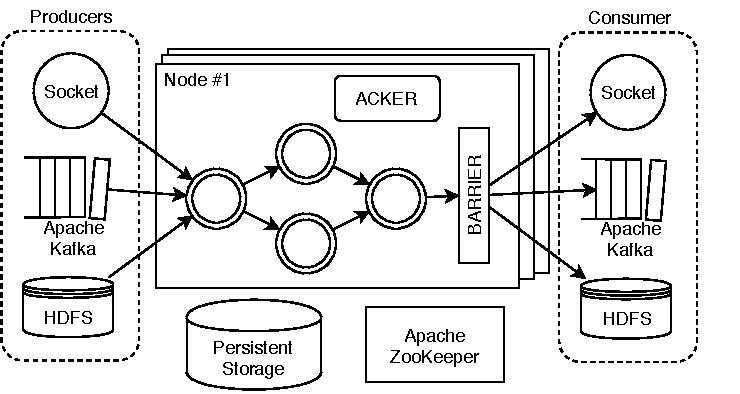
\includegraphics[width=0.70\textwidth]{pics/arch}
  \caption{The overall scheme of the system components}
  \label {system-architecture}
\end{figure}

\subsection{Ordering model}
The meta-information of data item is implemented as a tuple of a {\it global time}, a {\it trace}, {\it child ids} and a {\it tombstone flag}.

\[Meta := (GlobalTime, ChildIds[\:], Trace, IsTombstone)\]

Global time is assigned to data item once the item enters the system. It is a pair of logical time and the identifier of the front. The identifier is used to resolve time collisions within different fronts. It is important to notice that we do not rely on any clock synchronization between nodes. The only implication of the clock skew is the system degradation regarding latency: 1 ms of the fronts clock difference appends 1 ms to minimal latency.

Each map operation can produce multiple items from one.  An ordinal number, child id, is stored in the meta information to differentiate them. {\it ChildIds} is an array of child ids, that corresponds to all visited map operations.

The global time and child ids are enough to identify data item within a stream if all processing is done in-order. In this case, if we compare global time and child ids lexicographicaly the meta has the desired properties that were defined in section~\ref{model-section}. 

In order to filter out all invalid data at the barrier, there is a need to match tombstones with corresponding invalid items. However, if any grouping repairs happened during processing, multiple items with the same global time and child ids exist in the stream. To differentiate them without direct payload comparison, there is a {\it Trace} value stored in the meta-information. The trace is a xor of all physical operations' ids (random 64-bit identifier) visited by item so far. Invalid item and the corresponding tombstone go along the same path, because they have the same payload and the balancing functions are deterministic. Therefore, item and the corresponding tombstone can be revealed via trace matching. 

\label{mininal-time}

\subsection{Minimal time within stream}

To release an item from the barrier we need to ensure that there are no in-flight tombstones for that item, i.e., tombstones which have been already generated, but have not arrived at the barrier yet.

\newtheorem{minimal-time-claim}{Lemma}

\begin{minimal-time-claim}
For any data item $D$ let $\mathcal{G} (D)$ be its global time. 
  If data item $D$ has global time $\mathcal{G} (D) < \mathcal{G} (F)$ for each in-flight element $F$, 
  then all tombstones for that item had already arrived at the barrier.
\end{minimal-time-claim}

\begin{proof}
  Let $D_{tomb}$ be a tombstone for {\it D}. 
  According to the definition of the tombstone item, $\mathcal{G} (D_{tomb}) = \mathcal{G} (D)$, hence $D_{tomb}$ is not in-flight.
  
  New tombstones for $D$ cannot be generated because items with global time greater than $\mathcal{G} (D)$ cannot trigger repair that affects $D$,
  This implies that if the stream does not contain items $D\prime$ such that $\mathcal{G} (D\prime) \le \mathcal{G} (D)$, then all tombstones for $D$ had already arrived at the barrier. $\square$
\end{proof}

Therefore, to output an item from the barrier, we should ensure that there are no items in the stream with the global time less than or equal to the global time of this item.

To track the global time of in-flight items we adopt an idea of {\it acker task} inspired by Apache Storm~\cite{apache:storm}. Acker tracks data items using a checksum hash, called {\it XOR}. When the item is sent or received by an operation, its global time and checksum are sent to the acker. This message is called {\it ack}.
 Acker groups acks by a global time and xors received checksum hashes. 
When an item is sent and later received by the next operation, xoring corresponding {\it XOR}s would yield 0.

Acks are overlapped to nullify {\it XOR} only when an item arrives at the barrier. That is, ack for receive is sent only after both processing and the ack sending for the transformed item are done, as illustrated in Figure~\ref{acker}. This technique guarantees that the {\it XOR} for some global time is equal to zero only if there are no in-flight elements with such global time.

\begin{figure}[ht]
  \centering
  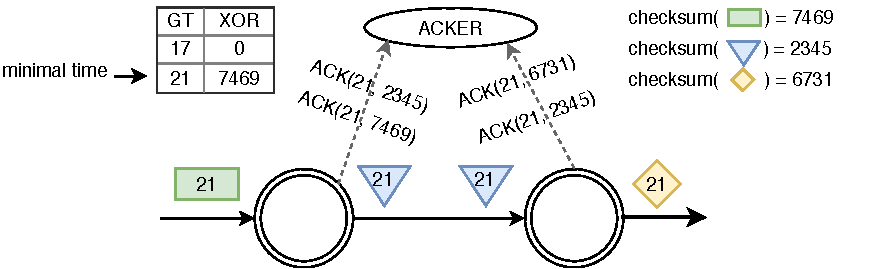
\includegraphics[width=0.8\textwidth]{pics/acker}
  \caption{The example of tracking minimal time using acker}
  \label {acker}
\end{figure}

The minimal time within a stream is the minimal global time with non-zero {\it XOR}. On minimal time changes, acker broadcasts the {\it new minimal time notification}. 
Therefore, the barrier can release elements with global time $\mathcal{G} (D)$ 
once it received notification with time greater than $\mathcal{G} (D)$.

To ensure that no fronts can generate item with the specific timestamp, each front periodically sends to acker a special message called {\it heartbeat} indicating that front will not issue items with a timestamp lower than the reported. The value in the ack table can become zero only after the corresponding heartbeat arrives.


\section {Experiments}
%%%% fs-run-time-experiments   Experiments

\label{fs-experiments-section}

\subsection{Setup}
We evaluated the series of experiments in order to estimate the performance of our system's prototype. As a stream processing task, we apply the computation of inverted index for Wikipedia documents. The computation of inverted index is implemented in terms of MapReduce transformations. We start with page mapping into the pairs {\it (word; word positions within the page)}. After that, word positions are reduced by word into the single structure. We assume the output of the stream to be change records of the inverted index structure, i.e. each input page triggers the output of the corresponding updates. 

Pairs {\it (word; word positions within the page)} must be ordered by page id and version before the update of inverted index state. Otherwise, it is possible to obtain the inconsistent index, if there are multiple versions of the same document.  
In the real-world, such scenario can be found in freshness-aware systems e.g. news processing engines. By the notion of {\it latency} we assume the time between two events: 
\begin{enumerate}
    \item Input page is taken into the stream
    \item All the change records for the page leave the stream
\end{enumerate}

In \FlameStream\ this algorithm is implemented as the typical conversion of MapReduce transformation, which is shown in section~\ref{fs-drifting}. Inverted index structure plays the role of an accumulator, and the accumulator map produces the most recent changes of this structure if any.

Our experiments were performed on the cluster of Amazon EC2 micro instances with 1GB RAM and 1 core CPU. We used 10000 Wikipedia articles as a dataset. 

\subsection{Overhead and scalability}

We take the ratio of arrived at the barrier items count to the number of the valid items among them as a key metric for the estimation of the overhead of our prototype. This value clearly represents the extra cost of our approach.

The relation between the number of workers, the delay between input documents and the proposed ratio is shown in Figure~\ref{overhead}. As expected, the peak of the ratio is achieved when the document per second rate is high, and the number of the nodes is low. This behavior can be explained by the fact that a few workers cannot effectively deal with such intensive load. Nevertheless, the proportion of invalid items reduces with the increase of workers number. Under non-extreme load, the total overhead of the optimistic approach is under 10\% for all considered number of workers. These results confirm that the ratio does not increase with the growth of the number of nodes.

\begin{figure}[htbp]
  \centering
  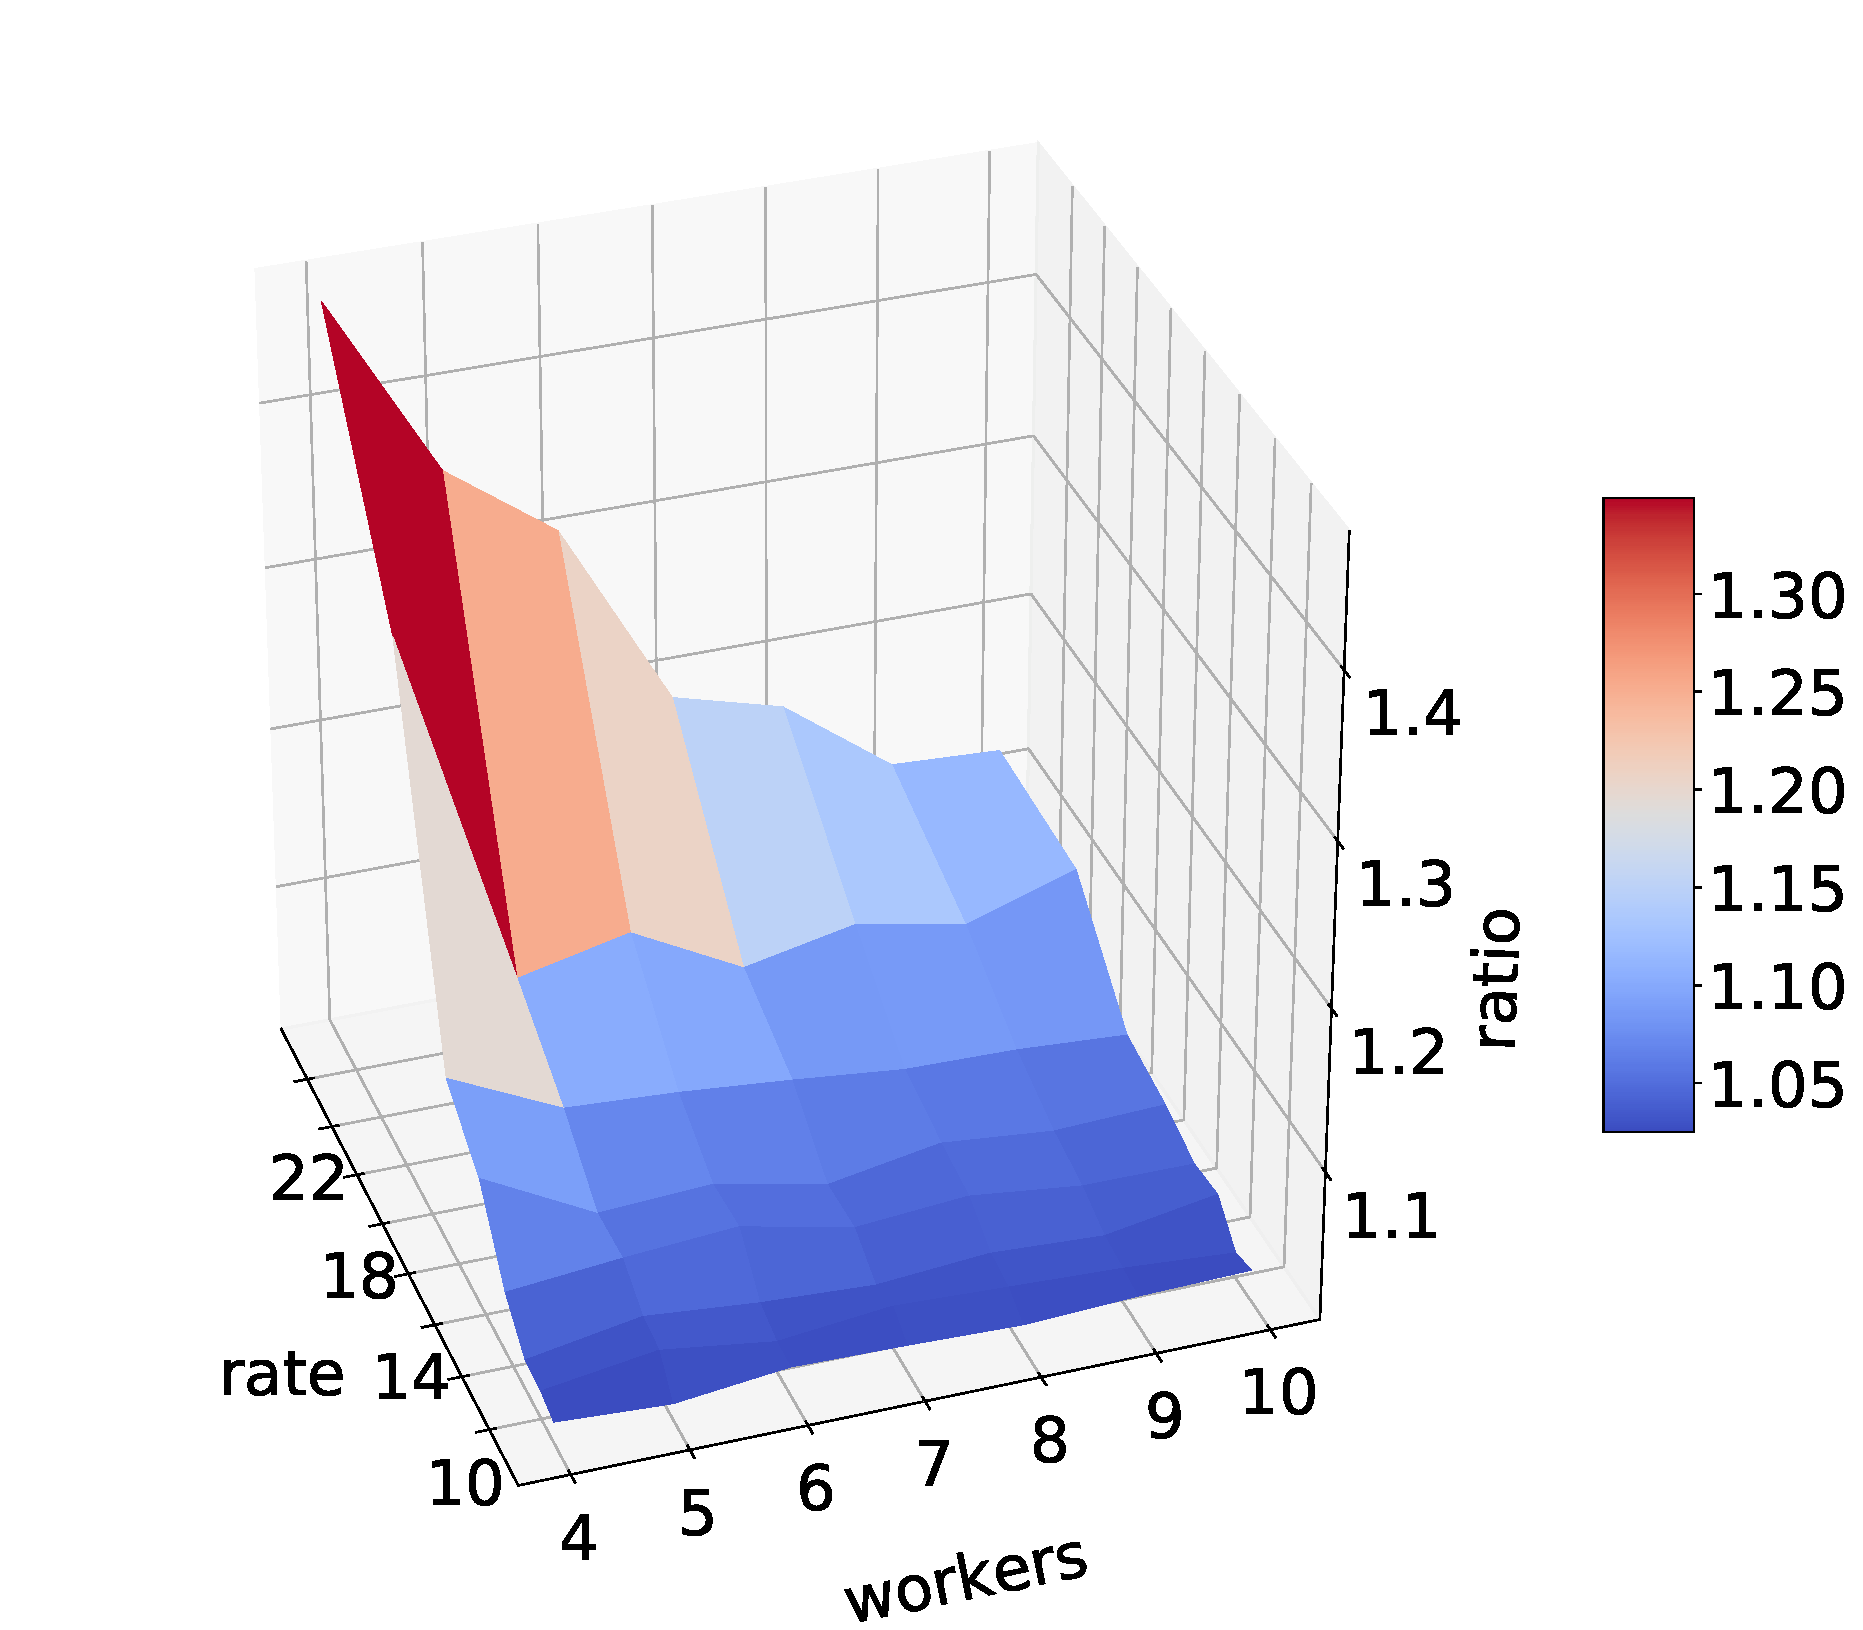
\includegraphics[width=0.5\textwidth]{pics/overhead}
  \caption{The relation between the number of workers, the delay between input documents and the replay ratio}
  \label {overhead}
\end{figure}

The latencies of \FlameStream\ across multiple workers for the fixed document rate of 70 ms are shown in Figure~\ref{fs-index-quantiles}. These figure demonstrate that latency is not significantly increased with the growth of the number of workers. 

Therefore, the most important conclusions of these experiments are: the proposed method is scalable, the overhead could be optimized by system setup.

\begin{figure}[htbp]
  \centering
  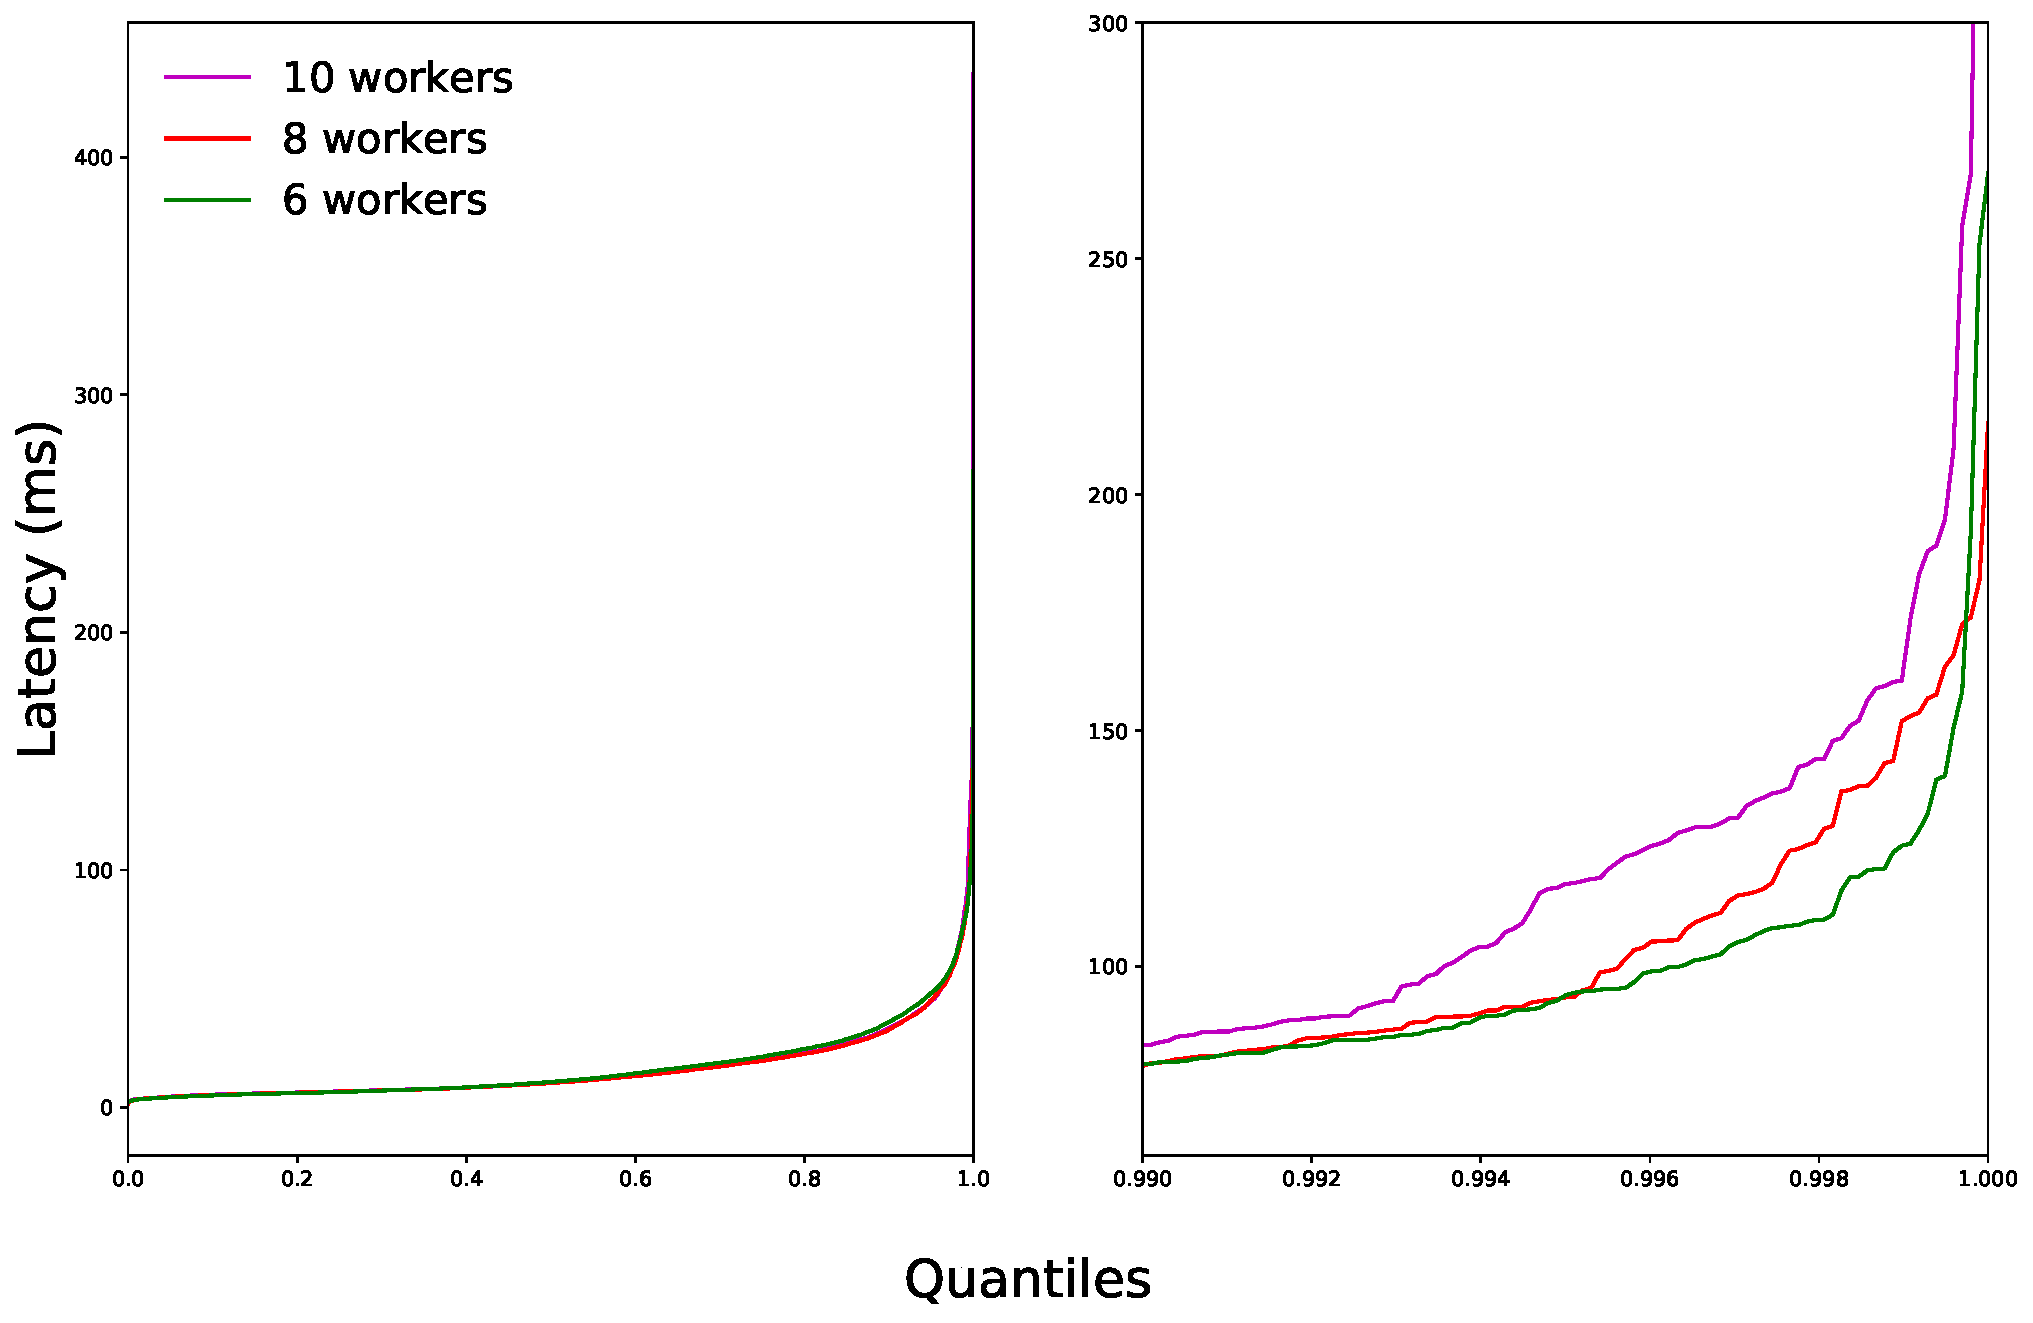
\includegraphics[width=0.48\textwidth]{pics/fs-index-quantiles}
  \caption{FlameStream latency distribution. Left - the whole distribution, right - tail latencies}
  \label {fs-index-quantiles}
\end{figure}

\subsection{Comparison against Apache Flink}

One of the most important goals of the experiments is the performance comparison with an industrial solution in terms of latency. Apache Flink is chosen for evaluation because it is state-of-the-art stream processing system that provides similar functionality and achieves low latency in the real-world scenarios~\cite{S7530084}. 

For Apache Flink, the algorithm for inverted index computation is adopted by the usage of {\it FlatMapFunction} for map step and stateful {\it RichMapFunction} for reduce step and for producing the change records. Order enforcing before reduce is implemented using custom {\it ProcessFunction} that buffers all input until corresponding low watermark is received. Watermarks are sent after each document. The network buffer timeout is set to 0 to minimize latency.

In this paper we compare $50^{th}$, $75^{th}$, $95^{th}$, and $99^{th}$ percentile of distributions, which clearly represent the performance from the perspective of the users' experience. Many papers report on averages, so these are included where it makes sense for comparison purposes. 

The comparison in latencies between \FlameStream\ and Flink within 10 nodes and distinct document rates is shown in Figure~\ref{fs-index-quantiles}. These results indicate that \FlameStream\ provides greater latency in the case of high load (25 rps). This fact corresponds with Figure~\ref{overhead}, which demonstrates that the overhead under such load is quite high. However, \FlameStream\ delivers better latency under less extreme loads. Firstly, the reason for such behavior can be the fact that Flink starts to update index only after the buffer before reduce stage is flushed. In contrast, \FlameStream\ flushes its barrier right before data is sent to a user, according to its optimistic nature. Secondly, low watermarks go along the stream and can be delayed by long-running operations, while acker processes ack messages independently. It is confirmed by Figure~\ref{buffer-vs-barrier}, which shows the comparison between waiting time in Flink's buffer and \FlameStream's barrier. 

\begin{figure}[htbp]
  \centering
  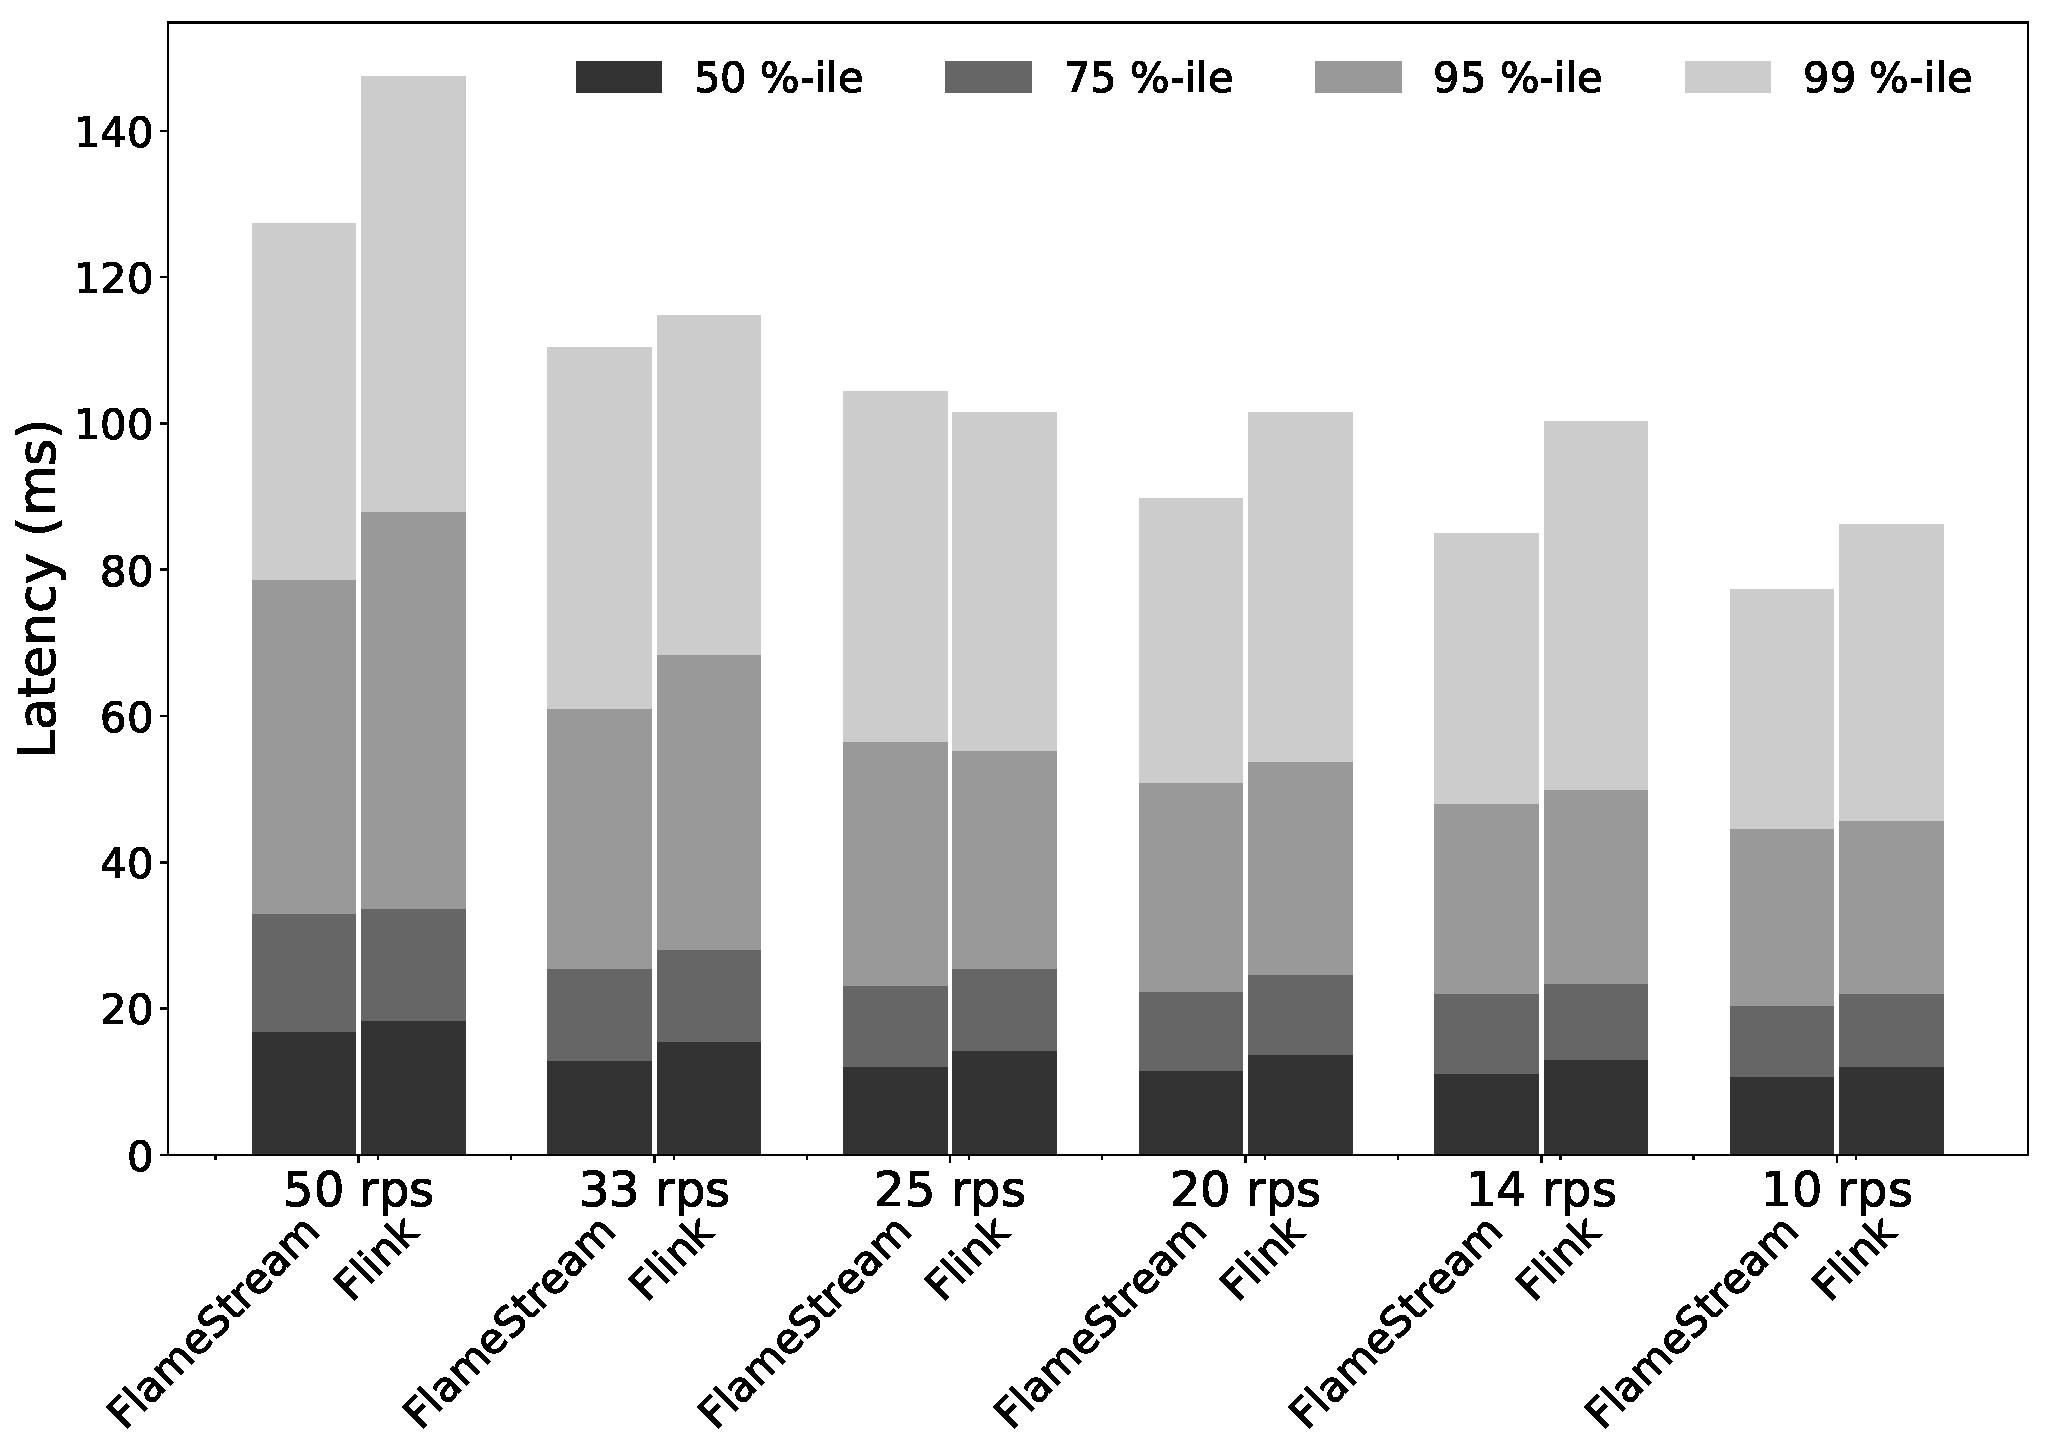
\includegraphics[width=0.5\textwidth]{pics/comp-index-quantiles}
  \caption{Latency comparison}
  \label {fs-index-quantiles}
\end{figure}

\begin{figure}[htbp]
  \centering
  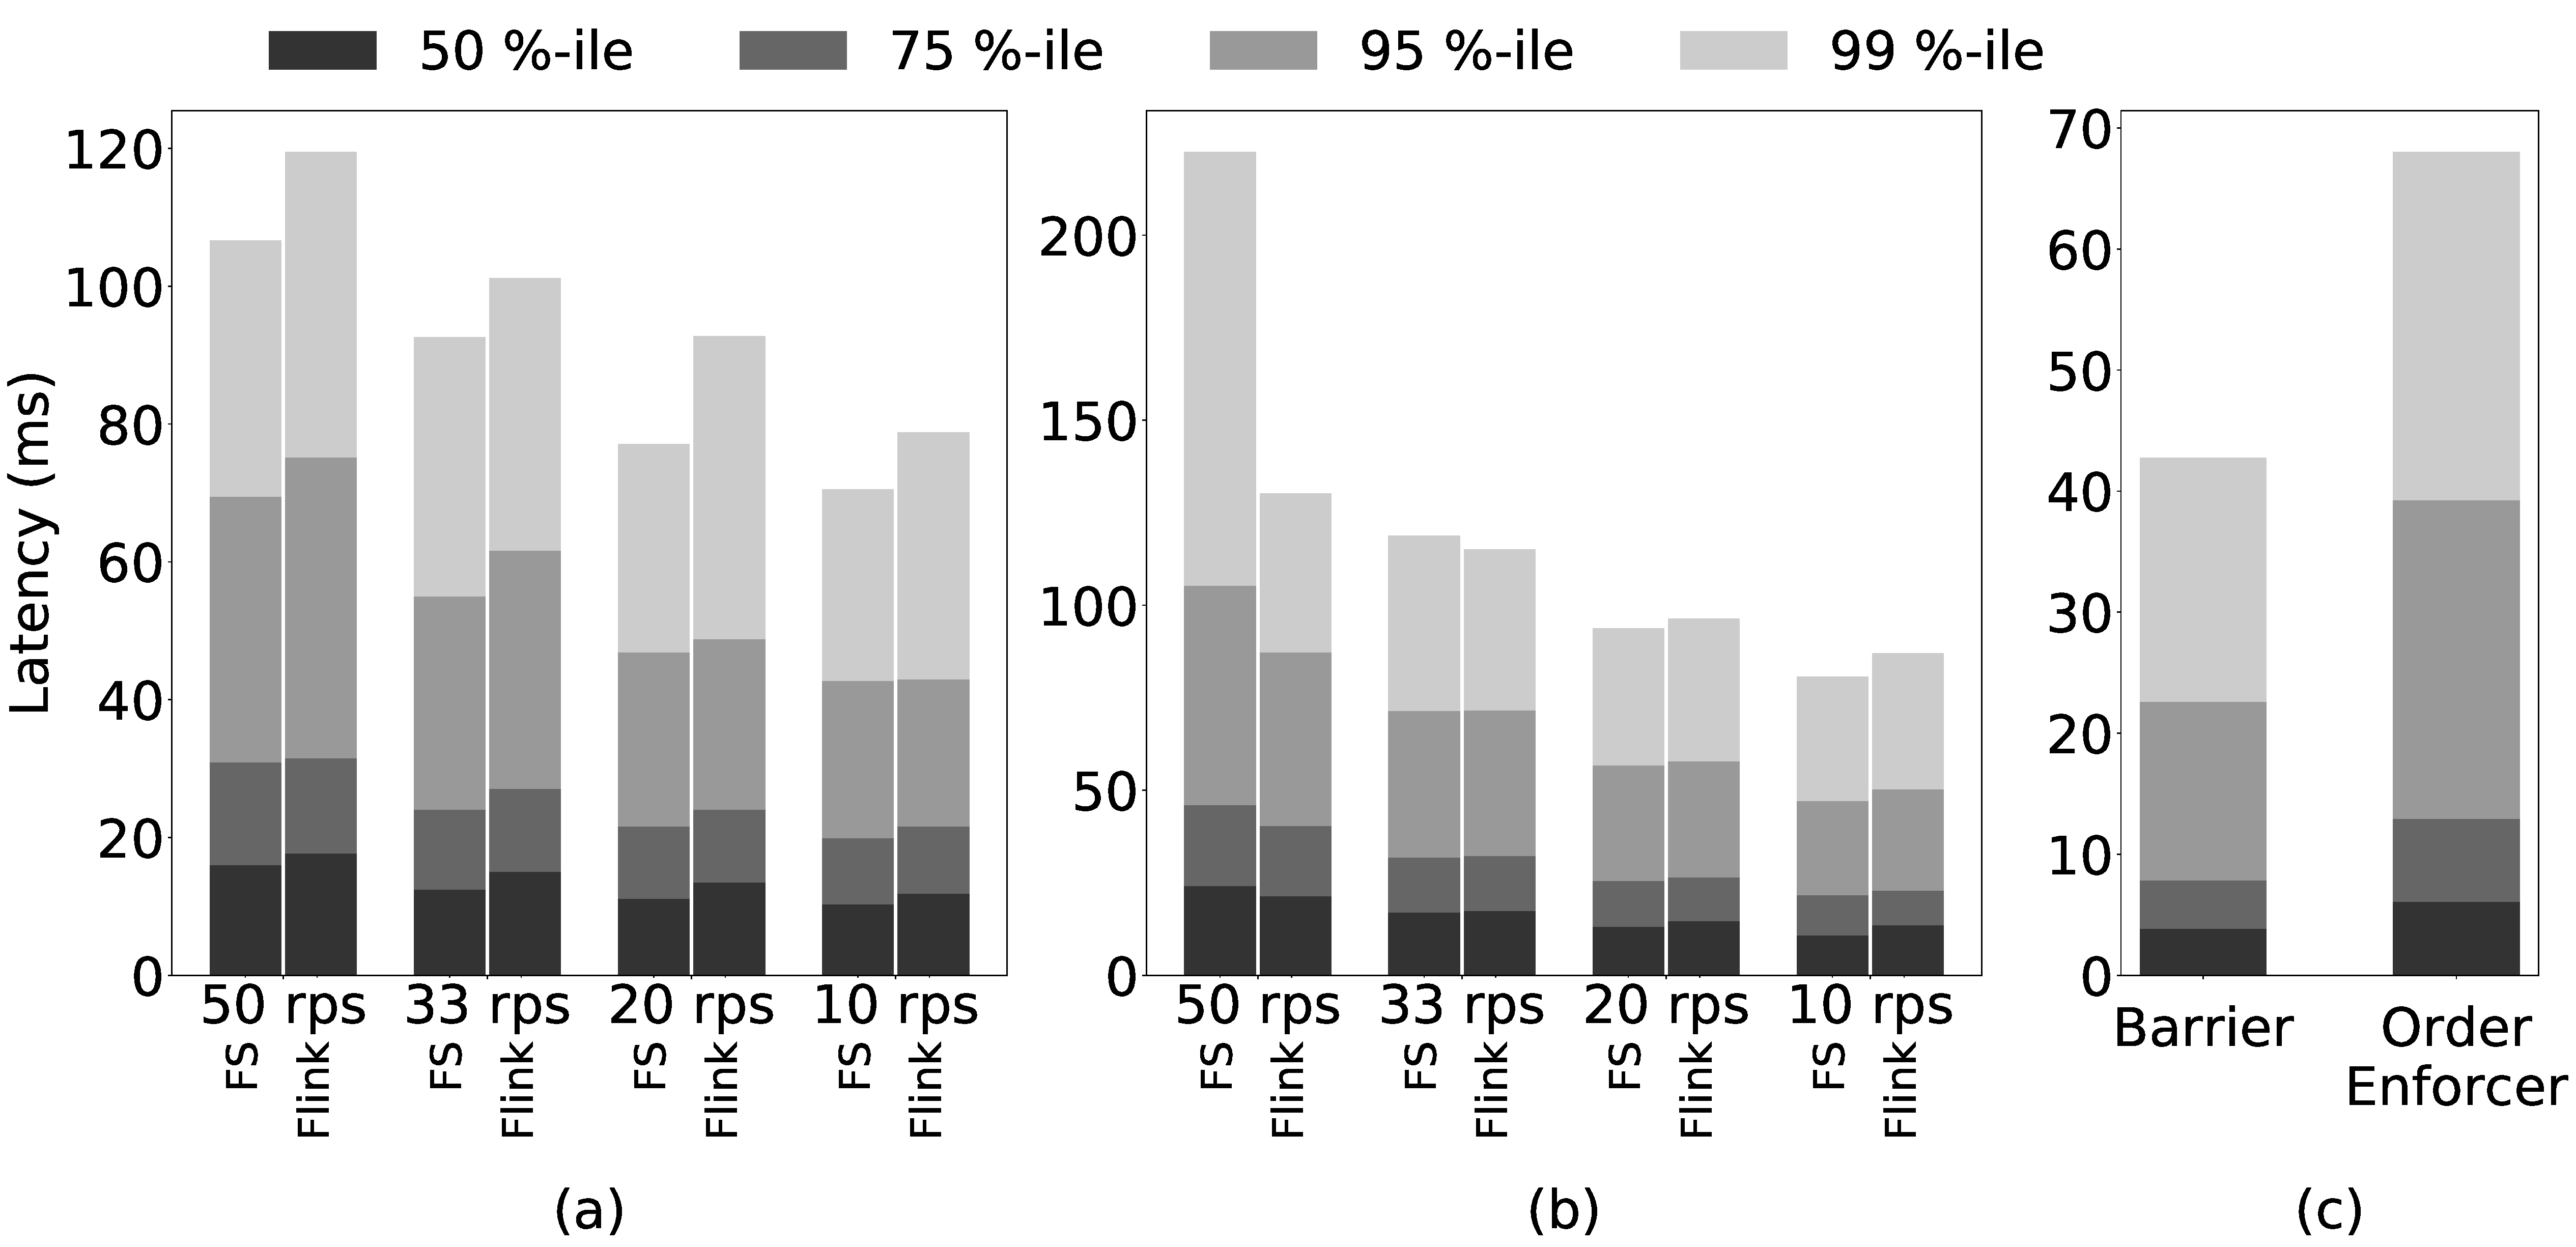
\includegraphics[width=0.25\textwidth]{pics/buffer-vs-barrier}
  \caption{Comparison between waiting time in Flink's buffer and FlameStream's barrier}
  \label {buffer-vs-barrier}
\end{figure}


\section {Related work}
%%%% fs-run-time-related  Related Work

\label {fs-related-section}

{\bf Data flow:}
One specific detail of our computational model is cyclic data flow graph support. Naiad~\cite{Murray:2013:NTD:2517349.2522738} by Microsoft Research provides an implementation of this idea. Nevertheless, Naiad applies cycles only for iterative computations and allows for each operation to have its own state. 

Another similar concept of Naiad is the usage of logical timestamps to monitor progress. However, to propagate the latest timestamp the pessimistic approach of notifications broadcasting is defined. Therefore, with the assumption of infrequent out-of-order items, our optimistic behavior is more relevant.

In our model, map and group operations are used as core processing primitives. Google Dataflow~\cite{Akidau:2015:DMP:2824032.2824076} provides the same idea. The primary distinction is that Google Dataflow model does not assume any kind of operation state. Additionally, this model provides different window types for grouping. FlameStream grouping is aligned with fixed-sized sliding window, but it is possible to implement other kind of windows by using cycle and grouping with window-affiliation hash.

{\bf State:}
The common approach to state management is to give a user the ability to handle a state of almost any supported operations. Such behavior is implemented, for isntance, in Apache Flink~\cite{carbone2015apache}, Storm~\cite{apache:storm}, Samza~\cite{Noghabi:2017:SSS:3137765.3137770}, Naiad~\cite{Murray:2013:NTD:2517349.2522738}.
To the best of our knowledge, FlameStream is the only open-source stream processing system that:
\begin{itemize}
    \item Stateless in terms of business-logic
    \item Supports any MapReduce transformations 
\end{itemize}

{\bf Tracking mechanisms within stream:}
One important task that FlameStream faces is handling of the minimal global time. In Apache Storm~\cite{apache:storm} acker is used to eliminate item traces. Unlike Strorm, we use acker to track the least global time of in-flight items and to detect package losses.


\section {Conclusion and future work}
%%% fs-run-time-conclu   Conclusions

\label {fs-conclusion-tection}

Some  of us are coders, but not writers.  Hopefully, almost everyone wil prove  the previos sentence is wrong.







\bibliographystyle{splncs03}
\bibliography{../../bibliography/flame-stream}

%\newpage
%\appendix
%\section{MapReduce transformation}
%%% It is just an empty TeX file.
%% Write your code here.

\label{fs-drifting}

Add bla-bla.

\subsection{MapReduce transformation}

TODO: rewrite. In this section, we demonstrate possible implementation of MapReduce-like transformation on a stream in order to show the soundness of our model. Map stage can be formulated in terms of our map operation. However, it is not obvious how to implement reduce stage, because it requires an explicit state handling. The algorithm~\ref{reduce} shows a generic reduce stage. The {\it accumulator} is an explicit state that should be maintained between subsequent iterations.

\begin{algorithm}
\caption{Generic reduce stage}
\label{reduce}
\begin{algorithmic}
  \Function{reduce}{$key$, $values$}
    \State $accumulator$ \Comment{reduce's state}
    \ForAll{$v \in values$} 
      \State \Call{combine}{$v$, $accumulator$}
    \EndFor
    \State \Return \Call{map}{$accumulator$}
  \EndFunction
\end{algorithmic}
\end{algorithm}

One possible way to implement reduce stage in our model is to make business logic state a part of the stream and work with it like with an ordinary data item. Figure~\ref{mapreduce-graph-figure} shows a generic graph for MapReduce transformation. Map and reduce parts are highlighted with a dashed line.

\begin{figure}[htb]
  \centering
  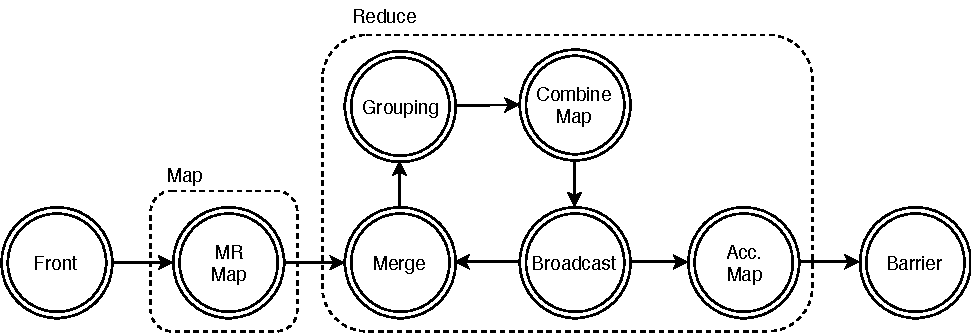
\includegraphics[scale=0.5]{pics/mapreduce}
  \caption{Logical graph for MapReduce transformations}
  \label {mapreduce-graph-figure}
\end{figure}

There are four types of data items in this stream: {\it input}, {\it mapped}, {\it accumulator}, {\it and reduced} items. Mapped, accumulator, and reduced items have the key-value structure of a payload. The operations of the stream have the following purposes:

\begin{itemize}
  \item The first map operation accepts input items and outputs mapped items according to map stage of MapReduce model
  \item The window of grouping is set to 2. It is used to group current accumulator with next data item in order to combine them together further. The hash function is designed to return distinct values for payloads with distinct keys
  \item The second map implements the actual combining. It accepts inputs that have a form of: \textit{(mapped item)} or \textit{(accumulator item, mapped item)}. The first kind is transformed into some initial value. The second one is combined into the new accumulator item as specified by reduce stage of MapReduce. The tuples with structure \textit{(mapped item, accumulator item)} are filtered out
  \item The third map is the accumulator map. It accepts accumulator items and applies the final map transformation to them
\end{itemize}

The key idea is that ordering assumptions about data items guarantees that each accumulator item always arrives at the grouping right after previous mapped item and before a new one. Hence, each mapped item that has not been combined yet would be grouped with the right accumulator item. Additionally, when combine map accepts tuple {\it (mapped item, accumulator item)}, then it means that mapped item was generated before accumulator item, and therefore, it had been already combined. The cycle gives the ability for new accumulator items to get back in the grouping operation. The accumulator map transforms the accumulator item into the final reduced item right before sink. Thereby, the stream reacts to each input item by generating new reduced item, which contains the actual value of the reduce stage.

\subsection{Example: word count}

We illustrate the MapReduce algorithm with an example of word counting. Map stage of this algorithm transforms each input word into key-value pair where the word is a key, and the value is 1. Reduce stage sums all values into the final result for the specific key. In this case the accumulator map is omitted, because the accumulator is the actual result of the reduce stage.

The example of input/output items, which are generated/ transformed by the part of the logical graph, is shown in Figure~\ref {word-count-figure}. According to our graph for MapReduce transformations, the item {\it m[dog, 1]} represents mapped item with key "dog" and value 1. The item {\it a[dog, 1]} describes accumulator item with key "dog" and value 1. Figure shows how the model reacts on two consequent input items containing word "dog". The meta-information of items is omitted for simplification. More precisely, there are 4 stages separated by dotted lines:

\begin{enumerate}
    \item New mapped item with key "dog" arrives at grouping with an empty state. Grouping outputs tuple with this single item. Combine map transforms it into the first accumulator item for key "dog" and value 1.
    \item The accumulator item arrives at grouping after it went through the cycle. It is grouped in the tuple with the mapped item that has been already in the state with key "dog". However, combine map drops this tuple, because of the order of items.
    \item New mapped item with key "dog" arrives at grouping. It is inserted right after the accumulator in the bucket for key "dog". The grouping operation outputs tuple containing the accumulator item and new mapped item. Map operation combines reduced and mapped items into new reduced items with key "dog" and value 2.
    \item New accumulator item arrives at grouping through the cycle, but new generated tuple is not accepted by combine map, as well as in step 2.
\end{enumerate}

\begin{figure}[htb]
  \centering
  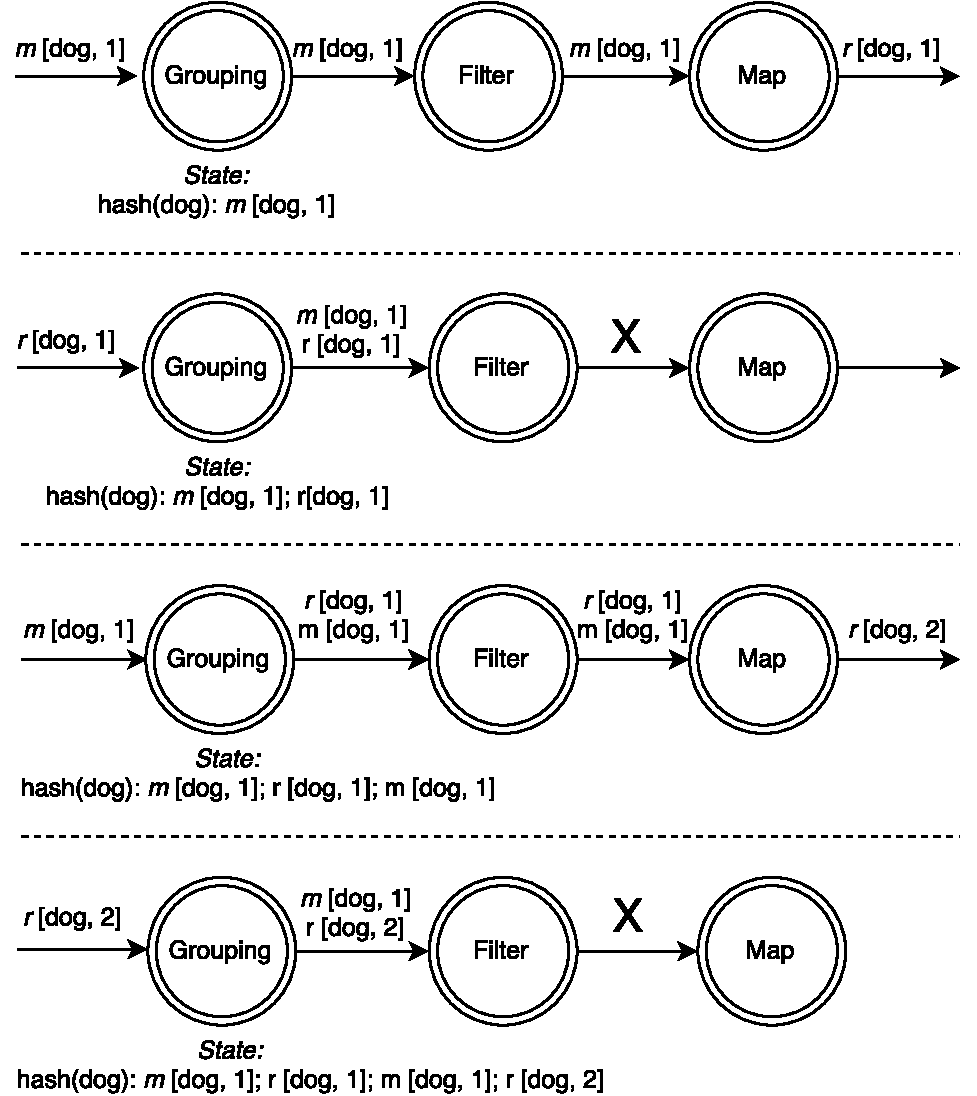
\includegraphics[scale=0.5]{pics/wordcount}
  \caption{Part of the stream evalutaion for word counting}
  \label {word-count-figure}
\end{figure}


\end {document}

\endinput
you can put whatever here
